\documentclass[12pt]{article}

\usepackage{estilo/sbc-template}
\usepackage{tikz}
\usepackage{transparent}
\usepackage{graphicx,url}
\usepackage[utf8]{inputenc}
\usepackage[brazil]{babel}
% para anotações no período de revisões
\usepackage{todonotes}
\usepackage{fancyhdr}
\usepackage{multirow}
\usepackage{scalefnt}
\usepackage{float}
\usepackage{datetime}
\usepackage{ifthen}
\usepackage[alf]{abntex2cite} 


% --------------------------------------
% Definições de formatação
% Númeração das páginas
\pagestyle{fancy}
\fancyhf{}
\fancyhead[R]{\thepage}
\renewcommand{\headrulewidth}{0pt}


\sloppy

% --------------------------------------
% Definições de informações do TCC
% --------------------------------------
\title{TÍTULO DO TRABALHO}

\author{NOME DO DISCENTE} %\inst{1}

\orientador{Prof. Título. Nome Completo}
% Caso não tenha coorientador, deixar o campo vazio.
\coorientador{}
% Caso tenha coorientador, descomentar linha abaixo.
%\coorientador{Prof. Título. Nome Completo}

\address{
  Curso de Bacharelado em Ciência da Computação\\ 
  Departamento de Ciência da Computação\\ 
  Universidade Federal de Roraima (UFRR)\\ 
  Boa Vista -- RR -- Brasil  
  \email{\{aluno\}@ufrr.br}
}
% --------------------------------------


% --------------------------------------
% Início do documento
% --------------------------------------
\begin{document} 

% Não é necessário alterar
% Capa personalizada para UFRR
\begin{titlepage}
    \begin{tikzpicture}[remember picture,overlay]
        \node[opacity=0.1,inner sep=0pt] at (current page.center){
            
\includegraphics[width=0.9\paperwidth]{estilo/dcc-logo.png}
        };
    \end{tikzpicture} 

    \begin{center}
        % Imagem no topo (troque o nome do arquivo para o correto)
        
\includegraphics[width=0.3\textwidth]{estilo/ufrr-logo.png} \\[2cm]

        % Instituição
        {\large
        UNIVERSIDADE FEDERAL DE RORAIMA\\
        CENTRO DE CIÊNCIAS E TECNOLOGIA\\
        DEPARTAMENTO DE CIÊNCIA DA COMPUTAÇÃO\\
        CURSO DE BACHARELADO EM CIÊNCIA DA COMPUTAÇÃO\\[3cm]
        }

        % Nome do aluno
        {\bfseries\Large Nome do Aluno}\\[1.5cm]

        % Título do trabalho
        {\bfseries\LARGE Título do Trabalho}\\[3.5cm]

        % Data
        {\large Boa Vista - RR\\
        Maio de 2025}
    \end{center}
\end{titlepage}

% Folha de rosto
%\newpage
\begin{titlepage}
    \begin{tikzpicture}[remember picture,overlay]
        \node[opacity=0.1,inner sep=0pt] at (current page.center){
            
\includegraphics[width=0.9\paperwidth]{estilo/dcc-logo.png}
        };
    \end{tikzpicture}
    \begin{center}
        % Título em negrito no topo
        {\bfseries\LARGE 
            \makeatletter
            \@title
            \makeatother
        }\\[4cm]

        % Nome do discente
        {\Large 
            \makeatletter
            \@author
            \makeatother
        }\\[4cm]

        % Texto com recuo à direita
        \begin{flushright}
            \parbox{9cm}{\setlength{\parindent}{0pt}
            Trabalho de Conclusão de Curso apresentado ao curso de Bacharelado em Ciência da Computação do Departamento de Ciência da Computação da Universidade Federal de Roraima, em cumprimento às exigências legais como requisito parcial à obtenção do título Bacharel em Ciência da Computação.
            }
        \end{flushright}

        \begin{flushright}
            \parbox{9cm}{\setlength{\parindent}{0pt}
            \textbf{Orientador:} Prof. Título. Nome Completo.
            }
        \end{flushright}

        \begin{flushright}
            \parbox{9cm}{\setlength{\parindent}{0pt}
            \textbf{Coorientador:} Prof. Título. Nome Completo.
            }
        \end{flushright}

        \vfill

        % Data ao final da página
        {\large Boa Vista - RR\\
        \today}
    \end{center}
\end{titlepage}


% Alterar texto ou suprimir
% Agradecimentos
% Este arquivo contém o conteúdo da página de agradecimentos do TCC.
%\newpage
\begin{titlepage}
    \begin{tikzpicture}[remember picture,overlay]
        \node[opacity=0.1,inner sep=0pt] at (current page.center){
            
\includegraphics[width=0.9\paperwidth]{estilo/dcc-logo.png}
        };
    \end{tikzpicture}
    \begin{center}
        % Título em negrito no topo
        {\bfseries\LARGE AGRADECIMENTOS}\\[4cm]

        % Texto de Agradecimentos
        {\bfseries\Large \todo[inline]{É opcional, mas é comum que se escreva esta seção de modo a reconhecer todos que contribuíram de modo relevante com a elaboração do TCC, sejam pessoas ou organizações. Exemplo: A todos os professores do curso que colaboraram e construíram bases sólidas no meu desenvolvimento e aprendizagem para o crescimento profissional. Seus nomes são inesquecíveis e por isso, dedico-lhes minha profunda admiração e respeito.}}

        

        \vfill

        % Data ao final da página
        {\large Boa Vista - RR\\
        \today}
    \end{center}
\end{titlepage}



% Sumário
\renewcommand{\contentsname}{\centering \bfseries SUMÁRIO}
\tableofcontents
\thispagestyle{empty}

\clearpage
\pagenumbering{arabic}


\maketitle


\begin{resumo} 
  \textcolor{red}{Comece com uma sentença apresentando o objetivo do estudo. Depois descreva o método. Passe para uma breve descrição de resultados, indicando, então, a conclusão do seu estudo. Finalize com uma frase que pode, por exemplo, convidar a comunidade científica para realizar mais estudos semelhantes ao seu ou que indique a contribuição do seu trabalho. O seu resumo deve ter, no máximo, 150 palavras ou 10 linhas. O mesmo vale para o abstract. Importante: em um resumo, tipicamente, não fazemos citações. Além disso, não se deve inserir fórmulas, equações, diagramas ou símbolos.}
\end{resumo}

% Resumo em inglês
\begin{abstract}
  \textcolor{red}{Dica para a produção de um resumo em inglês: traduza o texto em português com a ajuda do Google Tradutor. Depois use uma versão gratuita do Grammarly para avaliar a qualidade do texto. Aceite as sugestões desse software.}
\end{abstract}

\keywords{Word 1, Word 2, Word 3}


%--------------------------------------
% Seções do artigo
%--------------------------------------
\section{Introdução}
\label{sec:introducao}

\todo[inline]{\textbf{NOTA}: O texto aqui apresentado é apenas a informação sobre algumas regras, para o escrita do seu trabalho, o texto abaixo DEVE SER REMOVIDO.}

\textcolor{red}{A função da introdução é informar ao leitor o tema da pesquisa, destacar a sua relevância científica e/ou social, sendo finalizada com a descrição de como o TCC está organizado, ou seja, como está subdividido. É importante ressaltar que a introdução apresenta a visão geral do TCC. Ela precisa ser sedutora, de forma a mobilizar o leitor para seguir com a leitura. Apesar de ser o primeiro capítulo do trabalho, normalmente é o último a ser feito. O motivo é que só apresentamos aquilo que já escrevemos.}

\textcolor{red}{1) Comece com uma sentença descrevendo qual é o tema da sua pesquisa, já podendo indicar o que você pretende investigar. 2) Na sequência, você pode dar uma ideia muito geral do que tem sido investigado nesse tema e já passar para a apresentação dos motivos para a realização da pesquisa. Alternativamente, pode já começar pela motivação. Motivos são argumentos, isto é, justificativas que indicam por qual motivo a pesquisa foi realizada. Argumente, preferencialmente, com base em dados, números, de pesquisa por qual motivo esse tema é relevante para a ciência e/ou para a sociedade. O ideal seria ter de dois a três argumentos para justificar a importância da sua pesquisa. Use citações para sustentar os argumentos. Os seus argumentos também podem mostrar a relevância do tema a partir das implicações que ele possui para a sociedade.}

\textcolor{red}{3) Você deve, então, explicitar o que irá estudar dentro do seu tema, o que significa explicitar o seu problema de pesquisa. O problema pode ser apresentado de duas formas: como objetivo (verbo no infinitivo + complemento) ou como pergunta. No caso do TCC do DCC, vamos mesclar as duas estratégias, apresentando o objetivo geral do estudo e perguntas de pesquisa que, se respondidas, atendem ao objetivo geral.
[4) Finalize a introdução com a descrição das seções que compõem o seu trabalho.}

\textcolor{red}{Atenção com relação à estrutura explicada. De modo simples, ela propõe que você responda três perguntas, sendo uma resposta por parágrafo: 1) Qual é o tema da pesquisa e o que você irá estudar dentro dessa temática? 2) Quais os motivos que justificam o que você pretende estudar? 3) Como o seu TCC está organizado?}

\todo[inline]{\textbf{NOTA}: Qual o problema que você está tentando resolver através do trabalho? Quais as restrições de projeto envolvidas?}

O problema considerado neste trabalho é expresso na seguinte questão:

\todo[inline]{A pergunta de pesquisa precisa ser respondida para que o objetivo geral possa ser alcançado. Pensando nisso, elabore a sua questão. O seu principal compromisso na pesquisa é conseguir essa resposta. Você pode ter uma só pergunta ou mais. Relembrando: você precisará responder essas perguntas, portanto é razoável não escrever qualquer questão.}

O objetivo deste estudo é 
\todo[inline]{Preencher com texto iniciando com um verbo no infinitivo seguido de complemento. Escolha um dos seguintes verbos e complementos: “Conduzir revisão de literatura sobre…”, “Caracterizar a variável…”, “Descrever a variável…”, “Desenvolver sistema/aplicativo/aplicação/script…”, “Investigar validade…”, “Testar validade do modelo…”, “Testar a relação de associação entre as variáveis A e B”, “Testar a relação de determinação entre as variáveis A e B” etc.}

Visando contribuir com $\dots$, o contexto deste trabalho
está situado no uso de metodologias e técnicas de $\dots$
\todo[inline]{Você deve descrever a situação ou o contexto geral referente ao assunto em questão, devem constar informações atualizadas
visando a proporcionar maior consistência ao trabalho. Adicionalmente, uma breve descrição da solução proposta.}

\textbf{Organização do Trabalho.} As demais seções restantes são organizados da seguinte forma:
% 
Nos \textbf{Fundamentos Teóricos}, são apresentados os conceitos abordados neste trabalho, especificamente: \textcolor{red}{XXX, YYY, e ZZZ.}
%
Nos \textbf{Trabalhos Correlatos}, são analisados os trabalhos correlatos a solução proposta.
%
Na \textbf{Método da Solução Proposta}, é descrito as etapas de execução do método da solução proposta para \textcolor{red}{XXXX}.
%
No \textbf{Planejamento para Avaliação Experimental}, é apresentado o planejamento e projeto para execução da avaliação da solução proposta.
%
E por fim nas \textbf{Considerações Parciais}, apresenta-se as considerações parciais e análise das atividades já desenvolvidas.
%\section{Fundamentos Teóricos}
\label{sec:fundamentos}

\todo[inline]{Aqui você vai selecionar os principais termos técnicos que precisam ser esclarecidos para que o leitor compreenda o seu trabalho e, ainda, vai explicar a teoria que está adotando. Use referências clássicas, mas também referências dos últimos cinco anos. Explique apenas os termos cruciais para o seu trabalho. Procure ser tão conciso quanto possível nesta seção. Não use citações literais. Não use citações de citações.}


\subsection{Fundamentos 1}
\label{sec:fundamentos1}
\todo[inline]{Segue \textbf{um exemplo} de apresentação de código na linguagem de programação C que pode ser utilizado na apresentação de conceitos.}

\begin{figure}[thp]	
    \centering
    \begin{subfigure}{0.4\textwidth}
    \centering
    \begin{lstlisting}[language=C]       
double custo(double entrada)
{
  if (entrada < 0) 
  {
    return -1;
  }
  if ((entrada * 1.5) <= 0)) 
  {
    return -1;
  }
  if(entrada > 50) 
  {
    return 1.25*entrada;
  }
  return 1.5*entrada;
}
	\end{lstlisting}
    \caption{Código C}
  \end{subfigure}%    
  \begin{subfigure}{.05\textwidth}
    \hfill
  \end{subfigure}%    
  \begin{subfigure}{.4\textwidth}
    \centering
\begin{lstlisting}[language=C]   
TEST_CASE_1()
{
  double result;
  result = custo(0.49)
  assert(result == 0.735);
}
TEST_CASE_2()
{
  double result;
  result = custo(51)
  assert(result == 63.75);
}
\end{lstlisting}
  \caption{Código de Teste}
  \end{subfigure}%
  \caption{\label{fig:program_test} Exemplo de código}
\end{figure}


\subsection{Fundamentos 2}
\label{sec:fundamentos2}

\todo[inline]{Segue um exemplo de uso de figura}

A Figura~\ref{fig_grafico} apresenta uma imagem.

\begin{figure}[h!]    
	\begin{center}
	    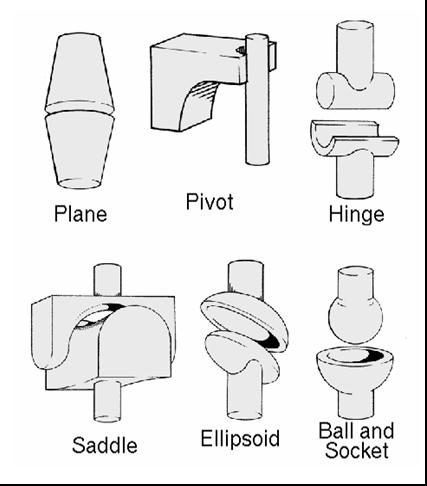
\includegraphics[scale=0.5]{imagens/fig2.jpg}
	\end{center}
    \caption{\label{fig_grafico}Descrição da iamgem.}
\end{figure}

\subsection{Fundamentos 3}
\label{sec:fundamentos3}

\todo[inline]{Segue um exemplo de uso referências.}

Segundo \citeonline{knuth:84}, tem-se que $\dots$ \cite{boulic:91} e \cite{smith:99}.

%--------------------------------------
% Referências
%--------------------------------------
\section{References}

Bibliographic references must be unambiguous and uniform.  We recommend giving the author names references in brackets, e.g. \citeonline{knuth:84},
\cite{boulic:91}, and \cite{smith:99}.

The references must be listed using 12 point font size, with 6 points of space before each reference. The first line of each reference should not be indented, while the subsequent should be indented by 0.5 cm.

%\bibliographystyle{estilo/sbc}
\bibliography{referencias}

%----------------------------
% Apêndice
% Capa personalizada para UFRR
\begin{center}        
    \vspace*{\fill}
    {\Huge \textbf{APÊNDICES}}\\
    \vspace*{\fill}
\end{center}

%------------------------------------------
% Apendice 1
%------------------------------------------
\section{APÊNDICE 01 – CRONOGRAMA DE EXECUÇÃO DA PESQUISA}
\label{sec:apendice-1}


\todo[inline]{Você pode cadastrar mais atividades. Para cada atividade, indique com um X nas colunas à direita o tempo que você irá precisar para finalizá-la.}

\begin{table}[H]
    \centering
    \begin{tabular}{|l|c|c|c|c|}
        \hline
        \multirow{2}{7.5cm}{\textbf{Atividades}} & \multicolumn{4}{c|}{\textbf{Período de execução da pesquisa}} \\ \cline{2-5}
        & \textbf{Mês 01} & \textbf{Mês 02} & \textbf{Mês 03} & \textbf{Mês 04} \\ \hline
        Atividade 01 & X & X & X & X \\ \hline
        Atividade 02 &   &   &   &   \\ \hline
        Atividade 03 &   &   &   &   \\ \hline
    \end{tabular}
\caption{Cronograma de Execução da Pesquisa}
\end{table}
    

% Anexo
% Capa personalizada para UFRR
\begin{center}        
    \vspace*{\fill}
    {\Huge \textbf{ANEXOS}}\\
    \vspace*{\fill}
\end{center}

%------------------------------------------
% Título: Anexo 01 - Termo de responsabilidade do discente
%------------------------------------------
\section{ANEXO 01 - TERMO DE RESPONSABILIDADE DO DISCENTE}
\label{sec:anexo-1}

\todo[inline]{Anexos são recursos que outro pesquisador produziu e que você usou no seu trabalho. Todos os alunos possuem, necessariamente, 03 anexos.}


\section{ANEXO 02 - DECLARAÇÃO DE AUTORIA}

\begin{center}
    \fontsize{12}{15}\selectfont
    \vspace*{0.5cm}
    \textbf{DECLARAÇÃO DE AUTORIA}
    \vspace*{1cm}
\end{center}

\vspace*{\fill}

Eu, \textbf{Nome completo do discente} (código de matricula \textbf{0000000000}), autor da monografia/TCC (Trabalho de Conclusão de Curso) sob o título \textbf{ ... }, declaro que o trabalho em referência é de minha total autoria e de minha inteira responsabilidade o texto apresentado. Declaro, ainda, que as citações e paráfrases dos  autores estão indicadas com as respectivas obras e anos de publicação. Declaro, para os devidos fins que estou ciente:
\begin{itemize}\setlength\itemsep{.02em}
    \item  dos Artigos 297 a 299 do Código Penal, Decreto-Lei n. 2.848 de 7 de dezembro de 1940;
    %
    \item  da Lei n. 9.610, de 19 de fevereiro de 1998, sobre os Direitos Autorais; e
    %
    \item  que plágio consiste na reprodução de obra alheia e submissão da mesma como trabalho próprio ou na inclusão, em trabalho próprio, de ideias, textos, tabelas ou ilustrações (quadros, figuras, gráficos, fotografias, retratos, lâminas, desenhos, organogramas, fluxogramas, plantas, mapas e outros) transcritos de obras de terceiros sem a devida e correta citação da referência.
\end{itemize}

O corpo docente responsável pela avaliação deste trabalho poderá  não  aceitar o referido trabalho caso os pontos mencionados acima sejam descumpridos, por conseguinte, considerar-me reprovado.

\vspace*{\fill}

\begin{center}
    \rule{7cm}{0.4pt} \\
    \fontsize{12}{15}\selectfont Assinatura do acadêmico(a) \\ 
    Boa Vista - RR, data (por extenso).
\end{center}

\vfill

\end{document}
